\documentclass[a4paper,11pt,bibliography=totoc,listof=totoc,headinclude=true,cleardoublepage=empty,oneside]{scrbook}
% Option "oneside" für einseitigen Druck. Weglassen, falls die Arbeit doppelseitig gedruckt wird

\usepackage[english,ngerman]{babel}
\usepackage[utf8]{inputenc}
%\usepackage{fullpage}
\usepackage{ifthen}
\usepackage{color}
\usepackage{amsmath,amsthm,amssymb,amsfonts}
\usepackage{graphicx}
\usepackage{psfrag}
\usepackage{algorithm}
\usepackage{algpseudocode}
\usepackage{float}

% links in pdf
\usepackage[unicode,colorlinks=true,pagebackref=false]{hyperref}

\newtheorem{theorem}{Theorem}[chapter]
\newtheorem{definition}[theorem]{Definition}
\newtheorem{cor}[theorem]{Corollary}
\newtheorem{rem}[theorem]{Remark}
\newtheorem{lemma}[theorem]{Lemma}
\newtheorem{prop}[theorem]{Proposition}

\newcommand{\R}{\mathbb{R}}
\newcommand{\N}{\mathbb{N}}
\newcommand{\Q}{\mathbb{Q}}
\newcommand{\Z}{\mathbb{Z}}
\renewcommand{\i}{\mathrm{i}}
\renewcommand{\Im}{\mathfrak{Im}}
\renewcommand{\Re}{\mathfrak{Re}}
\newcommand{\dff}{\Tilde{\beta}_\alpha}
\newcommand{\dffv}{\Tilde{\beta}_{\Vec{\alpha}}}
\newcommand{\bigO}{\mathcal{O}}
\newcommand{\F}{\mathcal{F}}
\newcommand{\e}{\mathrm{end}}

\algdef{SE}[DOWHILE]{Do}{doWhile}{\algorithmicdo}[1]{\algorithmicwhile\ #1}%


% Zum Druck verwende schwarze Links!
%\usepackage[unicode,colorlinks=true,linkcolor=black,citecolor=black,urlcolor=black,pagebackref=false]{hyperref} 
	% colorlinks=false umrahmt Links statt einzufaerben, 


% document style
\KOMAoptions{footinclude=false} % Fusszeile wird nicht zu Satzspiegel gezaehlt
\KOMAoptions{headsepline=true} % Trennlinie zwischen Kopfzeile und Text
\KOMAoptions{DIV=12} % beeinflusst Satzspiegel
\KOMAoptions{BCOR=8mm} % Bindekorrektur
\pagestyle{headings} % mit Kopfzeilen

\recalctypearea % berechne Satzspiegel neu

\definecolor{change}{rgb}{0,.55,.55}

\def\revision#1{{\color{red}#1}}


%%%%%%%%%%%%%%%%%%%%%%%%%%%%%%%%%%%%%%%%%%%%%%%%%%%%%%%%%%%%%%%%%%%%%%%%%%%%%%%%%%%%%%%%%%%%%%%%%%%%%%%%%%%%%%
%%%%%%%%%%%%%%%%%%%%%%%%%%%%%%%%%%%%%%%%%%%%%%%%%%%%%%%%%%%%%%%%%%%%%%%%%%%%%%%%%%%%%%%%%%%%%%%%%%%%%%%%%%%%%%
%%%%%%%%%%%%%%%%%%%%%%%%%%%%%%%%%%%%%%%%%%%%%%%%%%%%%%%%%%%%%%%%%%%%%%%%%%%%%%%%%%%%%%%%%%%%%%%%%%%%%%%%%%%%%%
%%%%%%%%%%%%%%%%%%%%%%%%%%%%%%%%%%%%%%%%%%%%%%%%%%%%%%%%%%%%%%%%%%%%%%%%%%%%%%%%%%%%%%%%%%%%%%%%%%%%%%%%%%%%%%

\begin{document}

%%%%%%%%%%%%%%%%%%%%%%%%%%%%%%%%%%%%%%%%%%%%%%%%%%%%%%%%%%%%%%%%%%%%%%%%%%%%%%%%%%%%%%%%%%%%%%%%%%%%%%%%%%%%%%
% TITELSEITE [OBLIGATORISCH]
%%%%%%%%%%%%%%%%%%%%%%%%%%%%%%%%%%%%%%%%%%%%%%%%%%%%%%%%%%%%%%%%%%%%%%%%%%%%%%%%%%%%%%%%%%%%%%%%%%%%%%%%%%%%%%

\pagenumbering{Alph}
\selectlanguage{ngerman}

\begin{titlepage}
  %\vspace*{-2cm}
  \begin{center}
    \includegraphics[width=0.45\textwidth]{TULogo.eps}
    \vskip 1cm%
    {\LARGE B~\Large A~C~H~E~L~O~R~A~R~B~E~I~T}
    \vskip 8mm
    {\huge\bfseries\color{change}Titel \\[1ex] ggf.\ mehrzeilig}
    \vskip 1cm
    \large 
    ausgef\"uhrt am    
    \vskip 0.75cm
    {\Large Institut f\"ur\\[1ex] Analysis und Scientific Computing}\\[1ex]
    {\Large TU Wien}
    \vskip0.75cm
    unter der Anleitung von
    \vskip0.75cm
    {\Large\bfseries 
Associate Prof. Dipl.-Math. Dr.rer.nat. Lothar Nannen \\ 
Univ.Ass. Dipl.-Ing. Dr.techn. Markus Wess}\\[1ex]
    \vskip 0.5cm
    durch
    \vskip 0.5cm
    {\Large\bfseries Michał Trojanowski}\\[1ex]
    Matrikelnummer: 12108865\\[1ex]
  \end{center}
  
  \vfill
  
  \small
  Wien, am \today
  \vspace*{-15mm}
\end{titlepage}

\cleardoublepage

%%%%%%%%%%%%%%%%%%%%%%%%%%%%%%%%%%%%%%%%%%%%%%%%%%%%%%%%%%%%%%%%%%%%%%%%%%%%%%%%%%%%%%%%%%%%%%%%%%%%%%%%%%%%%%
% DANKSAGUNG / ACKNOWLEDGEMENT [OPTIONAL]
%%%%%%%%%%%%%%%%%%%%%%%%%%%%%%%%%%%%%%%%%%%%%%%%%%%%%%%%%%%%%%%%%%%%%%%%%%%%%%%%%%%%%%%%%%%%%%%%%%%%%%%%%%%%%%

\chapter*{Danksagung} %\chapter*{Acknowledgement}
\thispagestyle{empty}
\selectlanguage{ngerman} %\selectlanguage{english}

{\color{change}
\begin{itemize}
\item auf Deutsch oder Englisch
\item Die Danksagung (engl. {\em Acknowledgement}) ist optional und kann auch entfallen. Denken Sie ggf.\ an Ihre eigenen Eltern!

\item Falls die Arbeit durch eine Forschungsprojekt finanziert wurde, so ist jedenfalls der Fördergeber (z.B.\ FWF oder WWTF) mit Projektnummer und Projektname zu nennen.
\begin{itemize}
\item siehe z.B.\ Dissertation von Michele Ruggeri:
\item[] \href{https://publik.tuwien.ac.at/files/publik_252806.pdf}{\ttfamily https://publik.tuwien.ac.at/files/publik\_252806.pdf}
\end{itemize}

\end{itemize}
}

\cleardoublepage

%%%%%%%%%%%%%%%%%%%%%%%%%%%%%%%%%%%%%%%%%%%%%%%%%%%%%%%%%%%%%%%%%%%%%%%%%%%%%%%%%%%%%%%%%%%%%%%%%%%%%%%%%%%%%%
% EIDESSTATTLICHE ERKLAERUNG [OBLIGATORISCH]
%%%%%%%%%%%%%%%%%%%%%%%%%%%%%%%%%%%%%%%%%%%%%%%%%%%%%%%%%%%%%%%%%%%%%%%%%%%%%%%%%%%%%%%%%%%%%%%%%%%%%%%%%%%%%%

\chapter*{Eidesstattliche Erkl\"arung}
\thispagestyle{empty}
\selectlanguage{ngerman}
\thispagestyle{empty}

\vspace*{2cm}

Ich erkl\"are an Eides statt, dass ich die vorliegende Bachelorarbeit selbstst\"andig und ohne fremde Hilfe verfasst, andere als die angegebenen Quellen und Hilfsmittel nicht benutzt bzw. die w\"ortlich oder sinngem\"a{\ss} entnommenen Stellen als solche kenntlich gemacht habe.

\vspace*{3cm}

\noindent
Wien, am \today
%
\hfill 
%
\begin{minipage}[t]{5cm}
\centering
\underline{\hspace*{5cm}}\\
\small{Michał Trojanowski}
\end{minipage}

\cleardoublepage

%%%%%%%%%%%%%%%%%%%%%%%%%%%%%%%%%%%%%%%%%%%%%%%%%%%%%%%%%%%%%%%%%%%%%%%%%%%%%%%%%%%%%%%%%%%%%%%%%%%%%%%%%%%%%%
% INHALTSVERZEICHNIS [OBLIGATORISCH]
%%%%%%%%%%%%%%%%%%%%%%%%%%%%%%%%%%%%%%%%%%%%%%%%%%%%%%%%%%%%%%%%%%%%%%%%%%%%%%%%%%%%%%%%%%%%%%%%%%%%%%%%%%%%%%

\pagenumbering{roman}
%\selectlanguage{ngerman} %
\selectlanguage{english} 

\tableofcontents

\cleardoublepage
\pagenumbering{arabic} 

%%%%%%%%%%%%%%%%%%%%%%%%%%%%%%%%%%%%%%%%%%%%%%%%%%%%%%%%%%%%%%%%%%%%%%%%%%%%%%%%%%%%%%%%%%%%%%%%%%%%%%%%%%%%%%
% EINLEITUNG / INTRODUCTION [OBLIGATORISCH]
%%%%%%%%%%%%%%%%%%%%%%%%%%%%%%%%%%%%%%%%%%%%%%%%%%%%%%%%%%%%%%%%%%%%%%%%%%%%%%%%%%%%%%%%%%%%%%%%%%%%%%%%%%%%%%

%%%%%%%%%%%%%%%%%%%%%%%%%%%%%%%%%%%%%%%%%%%%%%%%%%%%%%%%%%%%%%%%%%%%%%%%%%%%%%%%%%%%%%%%%%%%%%%%%%%%%%%%%%%%%%
%%%%%%%%%%%%%%%%%%%%%%%%%%%%%%%%%%%%%%%%%%%%%%%%%%%%%%%%%%%%%%%%%%%%%%%%%%%%%%%%%%%%%%%%%%%%%%%%%%%%%%%%%%%%%%
\chapter{Introduction}
\label{chapter:introduction}


\chapter{A Krylov eigenvalue solver based on filtered time domain solutions}
\label{chapter:ftd}
In this chapter, we present the concept of a Krylov eigenvalue solver for computing eigenvalues of the negative Laplace operator. By reformulating the problem to its weak form and selecting a finite solution space, we find that our problem is equivalent to a matrix eigenvalue problem for some high-dimensional matrix. The core idea of the Krylov eigenvalue solver is to construct a matrix $C$ that has the same eigenspaces as the original problem but different eigenvalues. Projection onto a lower-dimensional Krylov space generated by this matrix significantly reduces computational costs. We construct the operator $C$ by integrating in time a solution to the wave equation multiplied by some weight function. Proper selection of the weight function allows us to find eigenvalues of the original problem in the desired region. This chapter is based on \cite{nannen}.

\begin{definition}[Eigenvalue problem of the negative Laplace operator]\label{def:ev problem}
    Let $\Omega \subset \R^d$ for $d=2,3$ be a bounded domain with a Lipschitz boundary. We seek eigenvalues $\omega^2 \in \R_{+}$ and eigenfunctions $u\in H^1(\Omega)\backslash \{0\}$ of the negative Laplace operator with Neumann boundary conditions:
        \begin{align}\begin{split}\label{eq:ev problem}
              -\Delta u &= \omega^2 u \quad \text{ in } \Omega, \\
              \frac{\partial u}{\partial \nu} &= 0 \quad\text{ on } \partial\Omega.
        \end{split}\end{align}
    Here $\frac{\partial}{\partial\nu}$ denotes the normal derivative, and $H^1$ is the Sobolev space.
\end{definition}
Now we discretize the problem in space, fixing a partition $\mathcal{T}$ of $\Omega$. We introduce a discrete solution space as a finite-dimensional space of piecewise polynomials on $\Omega$.
\begin{definition}[Discrete solution space]\label{def:solution space}
Let $\mathcal{P}_p$ denote the space of polynomials up to degree $p \in \N$. We define the discrete solution space as
\begin{equation*}
V_h := \left\{v \in H^1(\Omega): \quad \forall T \in \mathcal{T}, \, v|_T \in \mathcal{P}_p \right\}
\end{equation*}
with finite dimension $N := \mathrm{dim} (V_h)$.
\end{definition}

Using Gauss's theorem, we can formulate both the weak and discrete forms of problem \eqref{eq:ev problem}.

\begin{definition}[Weak formulation of the eigenvalue problem]\label{def:weak form}
Let $\Omega$ be a bounded Lipschitz domain, as defined in Definition \ref{def:ev problem}, and $V_h$ be the discrete solution space. We seek eigenvalues $\omega_h^2 \in \R_+$ corresponding to discrete eigenfunctions $u \in V_h\backslash\{0\}$, such that for all test functions $\varphi \in V_h$, the following holds:
\begin{equation}\label{eq:weak form}
\int_\Omega \nabla u \cdot \nabla \varphi \, dx = \omega_h^2 \int_\Omega u \varphi \, dx.
\end{equation}
\end{definition}

To simplify notation in subsequent sections, we omit the index $h$ for discrete eigenfunctions and eigenvalues. We now demonstrate that the discrete eigenvalue problem \eqref{eq:weak form} reduces to a matrix eigenvalue problem, since the solution space is finite-dimensional.

\begin{definition}\label{def:SM matrices}
Let $V_h$ be an $N$-dimensional solution space with basis $(\varphi_1, \dots, \varphi_N)$. We define matrices $S:=(s_{ij})_{i, j=1}^N $ and $M:=(m_{ij})_{i, j=1}^N $ as follows:
\begin{equation*}
s_{ij} := \int_\Omega \nabla \varphi_i \cdot \nabla \varphi_j \, dx \quad \text{ and } \quad m_{ij} := \int_\Omega \varphi_i \varphi_j \, dx.
\end{equation*}
\end{definition}

\begin{lemma}
Equivalent to the problem stated in Definition \ref{def:weak form} is the eigenvalue problem to find non-trivial $v \in \R^N$ and $\omega^2 \in \R_+$ such that:
\begin{equation}\label{eq:matrix form}
Sv = \omega^2 Mv
\end{equation}
where $S, M \in \R^{N \times N}$ are defined in Definition \ref{def:SM matrices}.
\end{lemma}

\begin{proof}
Since $(\varphi_1, \dots, \varphi_N)$ forms a basis of $V_h$, it suffices, if \eqref{eq:weak form} holds for all basis functions. By representing $u$ with coordinate vector $v\in \R^N$, we can substitute $u = (\varphi_1, \dots, \varphi_N) v$. Thus, we obtain:
\begin{align*}
        \forall j=1, \dots, N : \, \int_\Omega (\nabla\varphi_1, \dots, \nabla\varphi_N)v\cdot \nabla \varphi_j \, dx &= \omega^2 \int_\Omega (\varphi_1, \dots, \varphi_N)v \varphi_j \, dx, \\
        \forall j=1, \dots, N : \, \int_\Omega (\nabla \varphi_j \cdot \nabla \varphi_1, \dots, \nabla \varphi_j \cdot \nabla \varphi_N) v \, dx &= \omega^2 \int_\Omega (\varphi_j\varphi_1, \dots, \varphi_j\varphi_N)v \,dx, \\ 
        \forall j = 1, \dots, N: \, (s_{j1},\dots,s_{jN})v &= \omega^2 (m_{j1},\dots, m_{jN})v,
\end{align*}
which is equivalent to \eqref{eq:matrix form}.
\end{proof}

\begin{rem}
Matrices $S$ and $M$ from Definition \ref{def:SM matrices} are self-adjoint. Furthermore, matrix $S$ is positive semi-definite and $M$ is positive-definite.
\end{rem}


\section{Elementary eigenvalue solvers for matrices}
Since we have approximated the eigenvalue problem of the negative Laplacian operator (see Definition \ref{def:ev problem}) into a matrix eigenvalue problem, we recall elementary numerical algorithms to solve such problems. For proofs of convergence of these algorithms, we refer to \cite{numericsAB}.

The first algorithm provides an approximation of an eigenvector corresponding to the eigenvalue with the largest absolute value among the eigenvalues of the matrix  under assumptions of Theorem \ref{theorem:power iteration}.

\begin{algorithm}[H]
\caption{Power iteration}\label{alg:power iteration}
\begin{algorithmic}
    \State \textbf{Input:} $A \in \R^{N \times N}$, start vector $v^{(0)}\in \R^N \backslash\{0\}$
    \For{$i = 1, 2, \dots$}
        \State $v \gets Av^{(i-1)} $
        \State $v^{(i)} \gets \frac{v}{\|v\|_2}$
    \EndFor
    \State \textbf{Output:} $v^{(i)}$ -- approximation of an eigenvector to the eigenvalue with the largest absolute value under assumptions of Theorem \ref{theorem:power iteration}.
    \end{algorithmic}
\end{algorithm}
\begin{theorem}\label{theorem:power iteration}
Let $A \in \R^{N \times N}$ be a diagonalizable matrix with eigenvalues $\mu_1, \dots, \mu_N$, such that $|\mu_1| > |\mu_2| \geq |\mu_j|$ for all $j = 3,\dots,N$. Let $(v_1, \dots, v_N)$ denote a basis of $\R^N$, such that for all $j=1, \dots N$, $v_j$ is a normed eigenvector to eigenvalue $\mu_j$. Let $v = \sum_{j=1}^N c_j v_j \in \R^N$ be a start vector, such that $c_1 \neq 0$. Then for all $i \in \N$, holds the error estimation for the eigenspace:
\begin{equation*}
        \left\| v^{(i)} - \frac{\mu_1^i c_1}{|\mu_1^i c_1|} v_1 \right\|_2 = \bigO\left( \left|\frac{\mu_2}{\mu_1}\right|^i\right) \text{ for } i \rightarrow \infty.
\end{equation*}
Furthermore, holds the error estimation for the convergence of the eigenvalue. Let $\mu^{(i)} := (Ax^{(i)})_k / x^{(i)}_k $ for some $k = 1, \dots, N$. It holds:
    \begin{equation*}
        |\mu_1 - \mu^{(i)}| = \bigO\left( \left|\frac{\mu_2}{\mu_1}\right|^i\right) \text{ for } i \rightarrow \infty.
    \end{equation*}
\end{theorem}
\begin{proof}
We refer to \cite[p. 116]{numericsAB}.
\end{proof}

The second algorithm enables us to compute the entire spectrum of a matrix under assumptions of Theorem \ref{theorem:QR alg}. 

\begin{algorithm}[H]
\caption{QR Algorithm}\label{alg:QR alg}
\begin{algorithmic}
    \State \textbf{Input:} $A \in \R^{N \times N}$
    \State $A^{(0)} \gets A$
    \For{$i = 1, 2, \dots$}
        \State compute QR-decomposition: $Q^{(i)} R^{(i)} = A^{(i-1)}$ 
        \State $A^{(i)} \gets R^{(i)}Q^{(i)}$
    \EndFor
    \State \textbf{Output:} $A^{(i)}$ -- approximation of an upper triangular matrix with eigenvalues of $A$ on the diagonal under assumptions of Theorem \ref{theorem:QR alg}. 
    \end{algorithmic}
\end{algorithm}

\begin{theorem}\label{theorem:QR alg}
    Let $A \in \R^{N \times N}$ be a diagonalizable matrix with pairwise different absolute values of eigenvalues: $\mu_1 > \mu_2 > \dots > \mu_N$. Let $\Lambda^{(i)} := \left(A^{(i)}_{11}, \dots, A^{(i)}_{NN}\right)$. Then $\Lambda^{(i)}$ converges linearly towards $(\mu_1, \dots, \mu_N)$ as $i\rightarrow\infty$. 
\end{theorem}

\begin{proof}
    We refer to \cite[p. 120]{numericsAB}.
\end{proof}

Since our goal is to find the eigenvalues of the negative Laplace operator, we could use the QR algorithm to obtain all eigenvalues of the discrete problem. However, this is not feasible due to the high computational costs of the QR algorithm. We focus on situations where the problem on the discrete level is high-dimensional. The QR algorithm demands the computation of a QR-decomposition of an $N \times N$ matrix in each iteration, which has cubic computational complexity. Therefore, this method is out of reach for our problem. We have to deploy a method that is based on a direct solver, such as the power iteration. 

\section{Krylov eigenvalue solver}

Now we need to make an assumption that there exists a matrix $C\in \R^{N \times N}$ such that its eigenvectors are linear combinations of eigenvectors of the discrete problem \eqref{eq:matrix form}. 

\begin{definition}\label{def:C}
    Let $C \in \R^{N\times N}$ be a matrix such that there exists an eigenvalue $\mu \in \R$ corresponding to the eigenvector $w\in \R^N$, i.e., $Cw = \mu w$, if and only if $w$ is an eigenvector or a linear combination of eigenvectors to some eigenvalue $\omega^2$ in the discrete problem \eqref{eq:matrix form}.
\end{definition}

We obtain properties of the matrix $C$ that will be needed. The exact choice and construction of this matrix will be discussed later. We recall the definition of a Krylov space.

\begin{definition}[Krylov space]
    Let $C \in \R^{N \times N}$ be a matrix and $r\in \R^N$ be a normalized start vector, i.e., $\|r\|_2=1$. For $m\in \N$, we define the Krylov space as a subspace of $\R^N$:
    \begin{equation*}
        \mathcal{K}_m(C; r) := \mathrm{span}\left\{r, Cr, \dots, C^{m-1}r\right\}.
    \end{equation*}
\end{definition}

In this thesis, we focus on situations where $N$ is large. Our goal is to project the $N$-dimensional eigenvalue problem \eqref{eq:matrix form} onto an $m$-dimensional Krylov space, using an orthonormal basis of this space. Typically, we choose $m$ much smaller than $N$, so that this problem is solvable with low computational costs using a direct solver.

Let $\mathcal{K}_m(C; r)$ be an $m$-dimensional Krylov space for matrix $C\in \R^{N\times N}$ and start vector $r\in \R^N$, where $\|r\|_2=1$. We obtain an orthonormal basis $(b_0, \dots, b_{m-1})$ of the Krylov space using Gram-Schmidt orthonormalization:
\begin{equation*}
    b_0 := r \quad \text{and} \quad \widetilde{b}_{j} := Cb_{j-1} - \sum_{i=0}^{j-1} (b_i^T C b_{j-1}) b_i, \quad b_j := \frac{\Tilde{b}_{j-1}}{\|\Tilde{b}_{j-1}\|_2} \quad \text{for all } j=1, \dots, m-1. 
\end{equation*}


Now we can project the original problem \eqref{eq:matrix form} onto the $m$-dimensional Krylov space.

\begin{prop}[Eigenvalue problem on Krylov space]
    Let $B_m = (b_0, \dots, b_{m-1}) \in \R^{N\times m}$ be an orthonormal basis of an $m$-dimensional Krylov space $\mathcal{K}_m(C; r)$. The eigenvalue problem on the Krylov space is to find eigenvalues $\omega_m^2 \in \R_+$ and eigenvectors $v_m\in\R^m$, such that:
    \begin{equation}\label{eq:Krylov problem}
        B_m^T S B_m v_m = \omega_m^2 B_m^T M B_m v_m.
    \end{equation}
\end{prop}
%TODO: proof????, Lemma? Theorem? 

Since matrices $S$ and $M$ are Hermitian, Krylov iteration leads to convergence of eigen-spaces of \eqref{eq:Krylov problem} towards the eigenspace of $C$ corresponding to the eigenvalue $\mu_{\max}$ with the largest absolute value. Obviously, projected eigenvalues $\omega_m^2$ converge towards the eigenvalue $\omega^2$ of the original problem \eqref{eq:matrix form} corresponding to $\mu_{\max}$.

To sum up the core idea of this section, we can explicitly formulate an (not yet implementable) algorithm based on Krylov spaces to compute eigenvalues $\omega^2$.

\begin{algorithm}[H]
\caption{Krylov eigenvalue solver}\label{alg:Krylov base}
    \begin{algorithmic}
        \State \textbf{Input:} matrix $C$, start vector $r$, $M^{-1}$, $S$, $m$ dimension of the Krylov space
        \State $b_0 \gets r$
        \For{$ k = 1, \dots, m-1$}
            \State $b_k \gets Cb_{k-1}$ \Comment{Krylov step}
            \State $b_{k} \gets b_k - \sum_{i=0}^{k-1} (b_i^T b_k) b_i$ \Comment{Gram-Schmidt orthogonalization}
            \State $ b_k \gets b_{k}/\|b_{k}\|_2 $\Comment{Normalization}
        \EndFor
        \State $B_m \gets (b_0, \dots, b_{m-1})$ \Comment{Projection matrix}
        \State $A \gets B_m^T M^{-1}S B_m$
        \State solve $Av = \omega_m^2 v$ with power iteration
    \end{algorithmic}
\end{algorithm}

Our goal is to compute eigenvalues $\omega^2$ of \eqref{eq:matrix form} in a given region of interest $\left[\omega_{\min}^2, \omega_{\max}^2\right]$. Therefore, we need matrix $C$ to fulfill the following four conditions.
\begin{itemize}
    \item $C$ satisfies the conditions in Definition \ref{def:C}.
    \item Eigenvalues $\mu$ corresponding to eigenspaces of eigenvalues $\omega^2$ in the region of interest have large absolute value.
    \item Eigenvalues $\mu$ corresponding to eigenspaces of eigenvalues $\omega^2$, which are not sought, are close to 0. 
    \item Each Krylov step $r \mapsto Cr$ can be computed with low cost.
\end{itemize}
In other words, the use of matrix $C$ filters sought eigenvalues from among all eigenvalues of the original problem \eqref{eq:matrix form} via common eigenspaces.

\begin{rem}
    Shift-and-inverse matrix:
    \begin{equation*}
        C_\rho := (S - \rho M)^{-1}M
    \end{equation*}
    for some $\rho \in \R$ has eigenvalue $\mu = (\omega^2 - \rho)^{-1}$ corresponding to the eigenspace to the eigenvalue $\omega^2$ of the original problem \eqref{eq:matrix form}. Therefore, $C_\rho$ with $\rho = (\omega^2_{\min}+\omega^2_{\max})/2 $ would be a possible choice of matrix $C$. Nevertheless, it requires the inverse of an $N\times N$ matrix $(S - \rho M)$, which for large $N$ is impossible with low computational complexity.
\end{rem}

\begin{proof}
    Let $(\mu, w)\in \R\times\R^N$ be an eigenpair of $C_\rho$. We note that $\mu \neq 0$, since matrices $(S-\rho M)^{-1}$ and $M$ have full rank. We have:
    \begin{align*}
        C_\rho w &= \mu w &&\iff \\
        (S - \rho M)^{-1}Mw &= \mu w  &&\iff \\
        \frac{1}{\mu}Mw &= (S - \rho M)w &&\iff \\
        Sw &= \underbrace{\left(\rho + \frac{1}{\mu}\right)}_{=\omega^2} Mw.&& 
    \end{align*}
    Therefore $\omega^2$ is an eigenvalue of $M^{-1}S$ to the eigenvector $w$. Conversely, if $\omega^2$ is an eigenvalue of $M^{-1}S$, then $\mu = (\omega^2 - \rho)^{-1}$ is an eigenvalue of $C_\rho$ to the same eigenvector. Obviously, $|\mu|$ takes on the largest values if $\omega^2 \approx \rho$.
\end{proof}

\section{Filtered time domain solutions}
To construct an appropriate finite-dimensional operator to replace the role of the matrix $C$ from the previous section, we proceed as follows. We consider the homogeneous wave equation with some initial condition $u_0 = (\varphi_1, \dots, \varphi_N)r$ projected onto our discrete solution space $V_h$ (see Definition \ref{def:solution space}). We discretize the problem in space and formulate its weak form. The evaluation of our operator $C$ at the point $r$ is a time-integral of the solution to this semi-discrete problem.

We consider the homogeneous 2- or 3-dimensional wave equation in $\Omega \times (0, \infty)$:
\begin{align}
\begin{split}\label{eq:wave equation}
    \ddot{u} = \Delta u \quad \text{in } \Omega \times (0, \infty), \quad  u = 0 \quad \text{in } \partial\Omega\times (0, \infty),\\
    u( \cdot, 0)= u_0, \quad \dot{u}(\cdot, 0) = 0 \quad \text{in } \Omega,
\end{split}
\end{align}
where $u$ is a function $\Omega \times [0, \infty) \rightarrow \R$ and $\ddot{u}$ denotes the second time-derivative.

\begin{prop}
    Let $V_h$ be a discrete solution space with basis $(\varphi_1, \dots, \varphi_N)$, and let $r$ denote the coordinate vector of the projection of $u_0$ onto $V_h$, i.e., $u_0 = (\varphi_1, \dots, \varphi_N)r$. Let $S$ and $M$ denote the matrices from Definition \ref{def:SM matrices}. Discretization in space of the problem \eqref{eq:wave equation} leads to the following linear system of ordinary differential equations:
    \begin{align}\label{eq:discr wave equation}
    \begin{split}
        M \ddot{y}(t; r) &= -S y (t; r) \quad \text{ for all } t \in (0, \infty) \\
        y(0; r) &= r, \quad \dot{y}(0; r) = 0. 
    \end{split}
    \end{align}
\end{prop}
\begin{proof}
    The theory of partial differential equations leads us to the ansatz $u(t, x) = \sum_{i=1}^\infty \kappa_i(t) \xi_i(x)$, where $\xi_i$ are the eigenfunctions of the negative Laplace operator \cite[p. 122]{Jungel}. Since we want to solve the problem in our solution space $V_h$, we can assume that $u(\cdot, t)=(\varphi_1, \dots, \varphi_N)y(t)$ for some vector-valued function $y: [0, \infty) \rightarrow \R^N$.

    We reformulate $\ddot{u} = \Delta u$ to its weak form:
    \begin{align*}
        \forall \varphi \in V_h : \, \int_\Omega \ddot{u} \varphi \, dx &= \int_\Omega \Delta u \varphi \, dx, \\
        \forall \varphi \in V_h : \, \int_\Omega \ddot{u} \varphi \, dx &= - \int_\Omega \nabla  u\cdot  \nabla \varphi \, dx.
    \end{align*}
    $V_h$ is a finite-dimensional space; therefore, the condition "for all test functions" is equivalent to the condition "for all basis test functions":
    \begin{align*}
        \forall j=1, \dots, N:\, \int_\Omega (\varphi_1, \dots, \varphi_N)\ddot{y} \varphi_j \, dx &= -  \int_\Omega (\nabla \varphi_1, \dots, \nabla \varphi_N)y\cdot  \nabla \varphi_j \, dx, \\
        M\ddot{y} &= -Sy.
    \end{align*}
    It remains to show the equivalence of initial conditions. For $u_0$, we have:
    \begin{equation*}
        (\varphi_1, \dots, \varphi_N)r = u_0 = u(\cdot, 0) = (\varphi_1, \dots, \varphi_N)y(0),
    \end{equation*}
    so $y(0) = r$ in $\Omega$, and similarly $\dot{y}(0) = 0$ in $\Omega$.
\end{proof}
Now we can solve the semi-discrete wave equation \eqref{eq:discr wave equation} to construct an integral operator. 
\begin{lemma}\label{lemma:y solution}
    The unique solution to \eqref{eq:discr wave equation} is:
    \begin{equation}\label{eq:solution wave eq}
        y(t; r) = \sum_{j=1}^N \cos(\omega_j t) (v_j^T r) v_j,
    \end{equation}
    where $(v_j)_{j=1}^N$ is an orthonormal basis of $\R^N$ of eigenvectors of matrix $M^{-1}S$ with corresponding eigenvalues $\omega_j^2$.
\end{lemma}
\begin{proof}
    Because of the symmetry of matrices $S$ and $M$, there exists an orthonormal basis $(v_j)_{j=1}^N$ of eigenvectors of $M^{-1}S$. We denote corresponding eigenvalues with $\omega_j^2$, $j=1, \dots N$. Obviously, for all $j=1, \dots, N$ and for all $c_{1j}, c_{2j}\in \R$, the function $t\mapsto \left(c_{1j} \cos(\omega_j t) + c_{2j} \sin(\omega_j t)\right)v_j$ solves the differential equation \eqref{eq:discr wave equation}. Due to the linearity of the problem, 
    \begin{equation*}
        y(t) = \sum_{j=1}^N \left(c_{1j} \cos(\omega_j t) + c_{2j} \sin(\omega_j t)\right)v_j
    \end{equation*}
    solves the differential equation. Initial values lead to the form \eqref{eq:solution wave eq}. The uniqueness of the solution follows from the Picard-Lindelöf theorem.
\end{proof}

Now we can define an integral operator that maps the initial value of the semi-discrete wave equation \eqref{eq:discr wave equation} to a weighted time-integral of its unique solution. The discrete form of this operator will take over the role of matrix $C$. Depending on the choice of the weight function, eigenvalues of this discrete operator may fulfill the requirements that we have set for matrix $C$ in the previous section. This will be discussed later in Chapter \ref{chapter:function}. 

\begin{definition}\label{def:pi_alpha}
    Let $\alpha: [0; \infty) \rightarrow \R$ be a piecewise continuous function with compact support. We define $\Pi_\alpha: \R^N \rightarrow \R^N$ as a linear operator:
    \begin{equation*}
        \Pi_\alpha r := \int_0^\infty \alpha(t) y(t;r) \,dt,
    \end{equation*}
    where $y(t;r)$ is the unique solution to \eqref{eq:discr wave equation} from Lemma \ref{lemma:y solution}.
\end{definition}

The following lemma determines the correspondence between eigenvalues of $\Pi_\alpha$ and eigenvalues of the original problem \eqref{eq:matrix form}.

\begin{lemma}
    Let $\beta_\alpha : [0, \infty) \rightarrow \R$ be a filter function defined by:
    \begin{equation}\label{eq:cont filter function}
        \beta_\alpha(\omega) := \int_0^\infty \alpha(t) \cos(\omega t) \,dt. 
    \end{equation}
    Then the following two statements hold.
    \begin{enumerate}
        \item If $\omega^2$ is an eigenvalue of \eqref{eq:matrix form} corresponding to eigenvector $v$, then $v$ is also an eigenvector of $\Pi_\alpha$ corresponding to eigenvalue $\beta_\alpha(\omega)$. 
        \item If $\lambda$ is an eigenvalue of $\Pi_\alpha$ to eigenvector $v$, then there exists an eigenvalue $\omega^2$ of \eqref{eq:discr wave equation} such that $\beta_\alpha (\omega) = \lambda$, and 
        \begin{equation*}
            v \in \bigoplus\{ U : \exists \omega \, U \text{ is eigenspace to eigenvalue to } \omega \text{ and } \beta_\alpha(\omega) = \lambda\}.
        \end{equation*}
    \end{enumerate}
\end{lemma}
\begin{proof}
    \begin{enumerate}
        \item Since $(v_j)_{j=1}^N$ is an orthonormal basis of eigenvectors of matrix $M^{-1}S$, every eigenvector of \eqref{eq:matrix form} equals $v_j$ from \eqref{eq:solution wave eq} for some $j=1, \dots, N$. Therefore $y(t, v) = \cos(\omega_j t)v$ and 
        \begin{equation*}
            \Pi_\alpha v = \int_0^\infty \alpha(t) \cos(\omega_j t) v \, dt = \beta_\alpha(\omega) v.
        \end{equation*}
        So the first claim holds.
        \item If $\lambda$ is an eigenvalue of $\Pi_\alpha$ with eigenvector $v$, then for all $k=1, \dots, N$ holds:
        \begin{align*}
             0 &= (\Pi_\alpha v - \lambda v)v_k = \int_0^\infty \alpha(t) \sum_{j=1}^N \cos(\omega_k t) (v_j^T v)\underbrace{(v_j^T v_k)}_{=\delta_{jk}} \, dt - \lambda v^Tv_k \\ &= \left(\int_0^\infty \alpha(t) \cos(\omega_kt) - \lambda \right)v_k^T v = (\beta_\alpha(\omega_k) - \lambda)v_k^T v.
        \end{align*}
        If $\beta_\alpha (\omega_k)\neq \lambda$, then $v_k^Tv = 0$. Therefore $v$ belongs to the sum of eigenspaces to eigenvalues such that $\beta_\alpha(\omega_k) = \lambda$. Moreover, $v$ is an eigenvector, so $v\neq 0$. Therefore, there exists at least one $k$ such that $v_k^T v \neq 0$, which implies $\beta_\alpha (\omega_k) = \lambda$. 
    \end{enumerate}
\end{proof}

\section{Time discretization}
In the previous section, we introduced an operator $\Pi_\alpha$ that could meet our eigenvalue requirements and replace the matrix $C$ in Krylov iteration. However, exact computation of the value $\Pi_\alpha r$ is impossible for two reasons: it demands an analytical solution $y(\cdot; r)$ to the semi-discrete wave equation \eqref{eq:discr wave equation} as well as the computation of an integral.

In numerical method, we replace the integral in the definition of $\Pi_\alpha$ by the rectangular rule. Since we only need the values of the function $y(\cdot; r)$ at quadrature nodes, we can discretize the problem \eqref{eq:discr wave equation} in time and compute an approximation of the exact solution at those points using the finite difference method.
\begin{lemma}[Finite difference method]\label{lemma:finite diffs}
    For a given function $y \in C^4 ([a, b])$ and a uniform mesh $(t_l := a+\tau l)_{l=0}^{L}$ with $L+1\in\N$ nodes and mesh-size $\tau = (a-b)/L$, for all $l=1, \dots, L-1$, we have:
    \begin{equation*}
        \ddot{y}(t_l) = \frac{y(t_{l+1}) - 2 y(t_l) + y(t_{l-1})}{\tau^2} + \bigO(\tau^2).
    \end{equation*}
\end{lemma}
\begin{proof}
    This follows from a straight-forward calculation using Taylor expansion of the function $y$. For details, see \cite[p. 93]{numodes}.
\end{proof}

\begin{prop}[Finite difference method for semi-discrete wave equation]
    Let $\tau>0$ be the step size of a uniform mesh on $[0, \infty)$. By replacing the second time derivatives in \eqref{eq:discr wave equation} with the finite differences from Lemma \ref{lemma:finite diffs}, we obtain the following approximation $y_l(r)$ of $y(\tau l; r)$ for all $l \in \N$:
    \begin{align}\label{eq:fd for wave eq}
    \begin{split}
        y_{l+1}(r) &:= -\tau^2M^{-1}S y_l(r) + 2y_l(r) - y_{l-1}(r) \quad \text{ for } l \in \N, \\
        y_{-1}(r) &:= y_0(r) := r.
    \end{split}
    \end{align}
\end{prop}
\begin{proof}
    For initial values, we have $y(0; r) = r = y_0(r)$. By Taylor expansion:
    \begin{equation*}
        y(-\tau, r) = y(0; r) - \tau \underbrace{\dot{y}(0; r)}_{=0} + \bigO(\tau^2) = r + \bigO(\tau^2) = y_{-1}(r) + \bigO(\tau^2).
    \end{equation*} 
    Replacing the second time derivative in \eqref{eq:discr wave equation} by finite difference leads to:
    \begin{align*}
        y(\tau(l+1); r) &- 2 y(\tau l; r) + y(\tau(l-1); r) = -\tau^2 M^{-1}S y(\tau l; r) + \bigO(\tau^4), \\
        y(\tau(l+1); r) &= -\tau^2 M^{-1}S y(\tau l; r) + 2y(\tau l; r) - y(\tau (l-1); r) + \bigO(\tau^4).
    \end{align*}
    Hence, $y_l(r)$ defined in \eqref{eq:fd for wave eq} approximates $y(\tau l; r)$ for all $l \in \N$.
\end{proof}

\begin{prop}[Discrete operator for Krylov iteration]\label{prop:C operator}
    Let $L \in \N$ be the number of quadrature nodes and $T>0$ be the upper bound of integration. Discretizing the operator $\Pi_\alpha$ (see Definition \ref{def:pi_alpha}) by the rectangular rule with step size $\tau = T/L$ and approximation $y(l\tau; r) \approx y_l(r)$ leads to the discrete operator $C : \R^N \rightarrow \R^N$:
    \begin{equation}\label{eq:C operator}
        r \mapsto Cr := \sum_{l=0}^{L-1} \tau \alpha(\tau l) y_l(r).
    \end{equation}
\end{prop}

The discrete operator $C$ defined in Proposition \ref{prop:C operator} allows us to avoid high computational costs in each Krylov step $r \mapsto Cr$. However, we have to verify the coincidence between eigenpairs of $C$ and eigenpairs of the original problem \eqref{eq:matrix form}. For this reason, we construct a discrete filter function as a discrete analogue of \eqref{eq:cont filter function}.

If $r$ is an eigenvector of the matrix $M^{-1}S$ with eigenvalue $\omega^2$, then the time-stepping \eqref{eq:fd for wave eq} takes the following form for all $n\in \N$:
\begin{equation}\label{eq:y_l q_l}
    y_l(r) = q_l(\omega)r  
\end{equation}
with $q_l(\omega)$ being the solution to the following recursion:
\begin{align}\label{eq:q def}
    \begin{split}
        q_{l+1}(\omega) &:= (2-\tau^2\omega^2) q_l(\omega) - q_{l-1}(\omega) \quad \text{ for } l \in \N,\\
        q_{-1}(\omega) &:= q_0(\omega) := 1.
    \end{split}
\end{align}
This linear difference problem has unique solution, which will be needed later in Lemma \ref{lemma:dff}. Therefore, we analyze the behavior of the solution as $l$ tends to infinity.

\begin{lemma}[Courant--Friedrichs--Lewy condition for $q_l$]\label{lemma:cfl}
    For a given $\tau > 0$ and $\omega > 0$, the unique solution to \eqref{eq:q def} is:
    \begin{equation}\label{eq:q explicit}
        q_l(\omega) =  \frac{c(\omega)-1}{2\i \Im(c(\omega))} c(\omega)^l + \frac{1 - \overline{c(\omega)}}{2\i \Im(c(\omega))}  \overline{c(\omega)}^l,
    \end{equation}
    where 
    \begin{equation*}
        c(\omega) := 1 - \frac{\tau^2 \omega^2}{2} + \i \sqrt{1 - \left(1 - \frac{\tau^2 \omega^2}{2}\right)^2}.
    \end{equation*}
    Therefore, if $\tau < 2/\omega$, then the CFL condition is satisfied and $|c(\omega)|=1$, implying the boundedness of $|q_l(\omega)|$ as $l \rightarrow \infty$. Otherwise, $|q_l(\omega)|$ is unbounded.
\end{lemma}
\begin{proof}
    The characteristic equation of the difference equation \eqref{eq:q def} is:
    \begin{equation*}
        c(\omega)^2 + (\tau^2\omega^2 - 2)c(\omega) + 1 = 0. 
    \end{equation*}
    If $\tau < 2/\omega$, then the solutions are:
    \begin{equation*}
        c(\omega) = 1 - \frac{\tau^2 \omega^2}{2} + \i \sqrt{1 - \left(1 - \frac{\tau^2 \omega^2}{2}\right)^2} \quad \text{ and } \quad \overline{c(\omega)} = 1 - \frac{\tau^2 \omega^2}{2} - \i \sqrt{1 - \left(1 - \frac{\tau^2 \omega^2}{2}\right)^2}.
    \end{equation*}
     Obviously, $|c(\omega)|=1$. Linearity of the recursion implies that the unique solution is given by $q_l(\omega) = C_1 c(\omega)^l + C_2 \overline{c(\omega)}^l$. From the initial values, we obtain a system of two equations for $C_1$ and $C_2$ with the solution:
    \begin{equation*}
        C_1 = \frac{c(\omega)-1}{2\i \Im(c(\omega))} \quad \text{ and } \quad C_2 = \frac{1 - \overline{c(\omega)}}{2\i \Im(c(\omega))}.
    \end{equation*}
    Therefore, representation \eqref{eq:q explicit} holds. If $\tau < 2/\omega$, then $\Re(c(\omega)) < 0$, and \eqref{eq:q explicit} remains bounded as $l\rightarrow \infty$. 
    
    Otherwise, if $\tau > 2/\omega$, then the roots of the characteristic equation are real:
    \begin{equation*}
        c(\omega) = 1 - \frac{\tau^2 \omega^2}{2} \pm \sqrt{\left(1 - \frac{\tau^2 \omega^2}{2}\right)^2 -1 }.
    \end{equation*}
    One of the roots is smaller than $-1$, so the solution to the linear difference equation cannot be bounded as $l\rightarrow\infty$.
\end{proof}

The matrix $M^{-1}S$ has spectral decomposition $M^{-1}S = V\mathrm{diag}(\omega_1^2, \dots, \omega_N^2)V^T$, thus there exists its square root $\sqrt{M^{-1}S} = V\mathrm{diag}(\omega_1, \dots, \omega_N)V^T$. 

\begin{lemma}\label{lemma:dff}
    Let $L\in \N$ be the number of quadrature nodes, $T$ be the upper bound of the integral, and $\tau = T/L$, as in Proposition \ref{prop:C operator}. Let $q_l(\omega)$ be defined for all $l \in \N$ and $\omega \in \R$ by \eqref{eq:q def}. We define the discrete filter function $\dff: [0, \infty) \rightarrow \R$ as follows:
    \begin{equation}\label{eq:dff}
        \dff(\omega) := \sum_{l=0}^{L-1} \tau \alpha(\tau l) q_l(\omega).
    \end{equation}
    \begin{enumerate}
        \item $\dff$ is a polynomial of degree $L-1$ in $\omega^2$.
        \item For $C$ defined in Proposition \ref{prop:C operator}, $C = \dff\left(\sqrt{M^{-1}S}\right)$.
        \item If $(\omega^2, v)$ is an eigenpair of the original problem \eqref{eq:matrix form}, then $(\dff(\omega), v)$ is an eigenpair of $C$.
        \item If $(\lambda, v)$ is an eigenpair of $C$, then there exists $\omega \in \R$ such that $\omega^2$ is an eigenvalue of \eqref{eq:matrix form}, $\dff(\omega)=\lambda$, and
        \begin{equation*}
            v \in \bigoplus\{ U : \exists \omega \, U \text{ is eigenspace to eigenvalue } \omega \text{ and } \dff(\omega) = \lambda\}.
        \end{equation*}
    \end{enumerate}
\end{lemma}
\begin{proof}
    The first claim follows directly from the construction of $q_l(\omega)$ \eqref{eq:q def}. Let $V: = (v_1, \dots, v_N)$ be an orthonormal basis of eigenvectors corresponding to eigenvalues $\omega_1^2, \dots, \omega_N^2$ of $M^{-1}S$. The spectral decomposition of $M^{-1}S$ is $M^{-1}S = V \mathrm{diag}(\omega_1^2, \dots, \omega_N^2) V^T$. Since \eqref{eq:fd for wave eq} is a linear difference equation, for arbitrary $r\in\R^N$ and for all $l\in \N$ we obtain:
    \begin{equation*}
        y_l(r) = y_l \left( \sum_{j=1}^N (r^T v_j)v_j \right) = \sum_{j=1}^N (r^T v_j)y_l(v_j) \stackrel{\eqref{eq:y_l q_l}}{=} \sum_{j=1}^N (r^T v_j)q_l(\omega_j)v_j.
    \end{equation*}
    Therefore, by the definition of $C$:
    \begin{align*}
        Cr &= \sum_{l=0}^{L-1} \tau\alpha(l\tau) y_l(r) = \sum_{j=1}^N \sum_{l=0}^{L-1} \tau\alpha(l\tau)q_l(\omega_j) (r^T v_j) v_j \\ &= \sum_{j=1}^{N}\dff(\omega_j)(r^Tv_j)v_j = V \mathrm{diag}\left(\dff(\omega_1), \dots, \dff(\omega_N)\right)V^Tr = \dff\left(\sqrt{M^{-1} S}\right)r.
    \end{align*}
    So the second statement holds. The third and fourth claims follow from the second one. Let $\dff(\omega) = \sum_{l=0}^{L-1} c_l \omega^{2l}$ for some $c_0, \dots, c_{L-1}\in \R$. If $v$ is an eigenvector of \eqref{eq:matrix form} to eigenvalue $\omega^2$, then:
    \begin{equation*}
        Cv = \dff\left(\sqrt{M^{-1}S}\right)v = \sum_{l=0}^{L-1} c_l (M^{-1}S)^{l}v = \sum_{l=0}^{L-1} c_l \omega^{2l}v = \dff(\omega)v,
    \end{equation*}
    so $\dff(\omega)$ is an eigenvalue of $C$ to $v$. If $(\lambda, v)$ is an eigenpair of $C$, then for all $k=0,\dots, N$ holds:
    \begin{align*}
        0 &= (Cv - \lambda v)v_k = \left(\left(\dff\left(\sqrt{M^{-1}S}\right)v_k\right)^Tv - \lambda v^T v_k\right) \\&= \dff(\omega_k)v_k^T v - \lambda v^T v_k = \left(\dff(\omega_k) - \lambda\right)v^T v_k.
    \end{align*}
    Since $v^Tv_k \neq 0$ for some $k=1, \dots, N$, it follows that $\lambda = \dff(\omega_k)$ and $v$ belongs to the sum of all eigenspaces corresponding to eigenvalues $\omega^2$, such that $\dff(\omega) = \lambda$.
\end{proof}

\section{Algorithm}
Now that we have constructed the operator $C$ meeting our requirements, we can reformulate Algorithm \ref{alg:Krylov base} into an implementable form.

\begin{algorithm}[H]
\caption{Krylov eigenvalue solver with filtered time-domain}\label{alg:Krylov pro}
   \begin{algorithmic}
        \State \textbf{Input: } weight function $\alpha$, start vector $r$ with $\|r\|_2 = 1$, $M^{-1}$, $S$, dimension $m$ of the Krylov space, time-step $\tau$, number of time-steps $L$
        \State $b_0 \gets r$
        \For{$k = 1, \dots, m-1$}\Comment{Krylov loop}
            \State $y_{-1}, y_{0} \gets r$
            \State $b_k \gets \tau \alpha(0) r$
            \For{$l = 1, \dots L-1$}\Comment{Time-stepping in each Krylov step}
                \State $y_l \gets -\tau^2 M^{-1}S y_{l-1} + 2y_{l-1} - y_{l-2}$ \Comment{$y_l$ represents $y_l(r)$ from \eqref{eq:fd for wave eq}}
                \State $b_k \gets b_k + \tau \alpha(\tau l)y_l$ \Comment{Computation of \eqref{eq:C operator}}
            \EndFor
            \State $b_k \gets b_k - \sum_{i=0}^{k-1}(b_i^Tb_k)b_i$ \Comment{Gram-Schmidt orthogonalization}
            \If{$\|b_k\|_2 \neq 0$}
                \State $b_k\gets b_k/\|b_k\|_2$ \Comment{Normalization}
            \Else
            \State $m\gets k$   \Comment{$b_k \in \mathrm{span}\{b_0, \dots, b_{k-1}\}$. Exact eigenspace is a subspace of $\mathcal{K}_k(C; r)$.}
                \State \textbf{break} 
            \EndIf
        \EndFor
        \State $B_m \gets (b_0, \dots, b_{m-1})$ \Comment{Projection matrix}
        \State $A \gets B_m^T M^{-1}S B_m$
        \State solve $Av_m = \omega_m^2 v_m$ with power iteration
    \end{algorithmic} 
\end{algorithm}

The chosen time-step $\tau$ should fulfill the CFL condition (see Lemma \ref{lemma:cfl}) for the largest absolute value among the eigenvalues $\omega^2$ of \eqref{eq:matrix form}. The computational complexity of this method depends on the number of time-steps $L$ (and thus by the end time of integration $T = \tau L$) and the dimension of the Krylov space $m$. Notice that in the presented algorithm, we can easily increase the dimension of the Krylov space without incurring significantly higher computational costs, since increasing $m$ by $\hat{m}$ requires only $\hat{m}$ additional iterations of the Krylov loop and solving the eigenvalue problem with power iteration. For more details about the stopping criterion, we refer to \cite[p. 8--9]{nannen}. In the next chapter, we will discuss the choice of the weight function $\alpha$.



\chapter{Choice of the weight function}
\label{chapter:function}
For the full functionality of the Krylov eigenvalue solver based on filtered time-domain we need appropriate weight function $\alpha$. First section of this chapter follows choice in \cite{nannen}. In subsequent sections we discuss other numerical methods of selection of the weight function.

The whole spectrum of eigenvalues $\omega^2$ of the discrete approximation \eqref{eq:matrix form} of the negative Laplacian eigenvalue problem is included in some interval $\left[0, \omega_\e^2\right]$. We search eigenvalues in given region of interest $\left[\omega_{\min}^2, \omega_{\max}^2\right]$. Deployed Krylov eigenvalue solver (Algorithm \ref{alg:Krylov pro}) allows us to compute eigenvalues $\omega^2$, such that absolute value of the discrete filter function $\left|\dff(\omega)\right|$ is maximal. 

Therefore our goal is to construct such weight function $\alpha$, that the filter function $\left|\beta_\alpha\right|$ \eqref{eq:cont filter function} or its discrete equivalent $\left|\dff\right|$ \eqref{eq:dff} takes on larger values, if $\omega \in \left[\omega_{\min}, \omega_{\max} \right]$ and is close to 0 otherwise. Of course, we can require this only in the controlled interval $\left[0, \omega_\e\right]$, since, according to Lemma \ref{lemma:dff}, $\dff$ is a polynomial. Moreover, we require, that the function $\alpha$ is piecewise continuous and compactly supported (see Definition \ref{def:pi_alpha}).

\section{Inverse Fourier transform method}
In this section we follow choice in \cite{nannen}. First presented method of selecting weight function bases on observation, that the mapping $ \alpha \mapsto \beta_\alpha$ is somehow similar to the Fourier transform. 
\begin{lemma}\label{lemma:alpha fourier}
    Let $\alpha$ be piecewise continuous weight function, such that $\alpha \in L^1\left([0, \infty)\right)$. Let $\hat{\alpha}: \R \rightarrow \R$ denote its symmetric extension, i.e., $\hat{\alpha}(-t) := \alpha(t)$ for all $t\in \R_+$. Then, for all $s\in \R$:
    \begin{equation*}
        \beta_\alpha (s) = \sqrt{\frac{\pi}{2}} \F\left[\hat{\alpha}\right] (s),
    \end{equation*}
    where $\mathcal{F}$ denotes the Fourier transform and $\beta_\alpha$ denotes the filter function  defined in \eqref{eq:cont filter function}.
\end{lemma}
\begin{proof}
    Obviously, if $\alpha \in L^1\left([0, \infty)\right)$, then $\hat{\alpha} \in L^1\left(\R\right)$. From \eqref{eq:cont filter function} follows:
    \begin{align*}
        \beta_\alpha (s) &= \int_0^\infty \alpha(t) \cos(s t) \,dt = \frac{1}{2}\int_{-\infty}^\infty \hat{\alpha}(t) \cos(s t) \,dt + \frac{\i}{2} \underbrace{\int_{-\infty}^\infty \hat{\alpha}(t) \sin(-st) \,dt}_{=0} \\&= \frac{1}{2} \int_{-\infty}^{\infty} \hat{\alpha}(t) e^{-\i st} \, dt = \sqrt{\frac{\pi}{2}} \F\left[\hat{\alpha}\right] (s).
    \end{align*}
    The sine-integral is 0, since $\hat{\alpha}$ is an even function and $t \mapsto \sin(-st)$ is an odd function. 
\end{proof}

This motivates the choice of the function $\alpha$ as truncated inverse Fourier transform. As goal function to be filter function $\beta_\alpha$ we choose symmetrical indicator function of the region of interest: $\chi_{\left[-\omega_{\max}, -\omega_{\min}\right]\cup\left[\omega_{\min}, \omega_{\max}\right]}$. Thanks to the symmetry of this function, its inverse Fourier transform is real-valued.

\begin{theorem}
    Truncation of the scaled inverse Fourier transform of the symmetric indicator function $\chi_{\left[-\omega_{\max}, -\omega_{\min}\right]\cup\left[\omega_{\min}, \omega_{\max}\right]}$ to a compact interval $[0, T]$, $T>0$, leads to following weight function:
    \begin{equation}\label{eq:alpha fourier}
        \alpha(t) = \begin{cases}
            \frac{2\left(\omega_{\max} - \omega_{\min}\right)}{\pi}, \quad & t = 0, \\
            \frac{4}{\pi t} \sin\left(\frac{t}{2}\left(\omega_{\max}-\omega_{\min} \right)\right)\cos\left(\frac{t}{2}\left(\omega_{\max}+\omega_{\min} \right)\right), \quad & t \in (0, T], \\
            0, \quad & \text{else.}
        \end{cases}
    \end{equation}
\end{theorem}
\begin{proof}
    Following Lemma \ref{lemma:alpha fourier} we compute:
    \begin{align*}
        \sqrt{\frac{2}{\pi}} \F^{-1}\left[\chi_{\left[-\omega_{\max}, -\omega_{\min}\right]\cup\left[\omega_{\min}, \omega_{\max}\right]}\right](t) &= \frac{1}{\pi} \int_{-\infty}^\infty \chi_{\left[\omega_{\min}, \omega_{\max}\right]} e^{\i st} \, ds \\ 
        & = \frac{1}{\pi} \left( \int_{-\omega_{\max}}^{-\omega_{\min}} \cos(st) \, ds + \int_{\omega_{\min}}^{\omega_{\max}} \cos(st) \, ds\right) \\ &+ \frac{\i}{\pi} \underbrace{\left(\int_{-\omega_{\max}}^{-\omega_{\min}} \sin(st) \, ds + \int_{\omega_{\min}}^{\omega_{\max}} \sin(st) \, ds \right)}_{=0} \\
        &= \frac{2}{\pi}\int_{\omega_{\min}}^{\omega_{\max}} \cos(st) \, ds \\
        &= \frac{2}{\pi t} \left(\sin\left(t\omega_{\max}\right) - \sin\left(t\omega_{\min}\right)\right) \\
        &= \frac{4}{\pi t} \sin\left(\frac{t}{2}\left(\omega_{\max}-\omega_{\min} \right)\right)\cos\left(\frac{t}{2}\left(\omega_{\max}+\omega_{\min} \right)\right).
    \end{align*}
    Obtained function is real-valued, but does not have compact support. Therefore we truncate it to finite interval $(0, T]$ and set $\alpha|_{(T, \infty)} := 0$. Since the limit from the right as $t\rightarrow 0^+$ is finite, we can right-continuously in 0 extend the function to interval $[0, \infty)$. This leads to representation \eqref{eq:alpha fourier}.
\end{proof}

Since the discretization \eqref{eq:dff} of the filter function $\beta_\alpha$ truncates time-interval, we truncate weight function $\alpha$ to the same time $T>0$, as assumed in $\dff$. Of course, replacing exact improper integral in definition of $\beta_\alpha$ \eqref{eq:cont filter function} by quadrature rule on finite time-interval impacts the function and therefore the discrete filter function $\dff$ can not be exact assumed target indicator function $\chi_{\left[\omega_{\min}, \omega_{\max}\right]}$. However, for our purposes it is sufficient, if $\dff$ takes on larger values in region of interest $\left[\omega_{\min}, \omega_{\max}\right]$ and is close 0 otherwise. 

Computational costs of the Krylov eigenvalue solver depend on number of time-steps $L=T/\tau$. CFL condition (see Lemma \ref{lemma:cfl}) allows us to choose time-step maximal as $\tau = 2/\omega_{\e}$. 

We choose setup in \cite[section 3.1.2]{nannen}: $\tau = 0.0056$, $\omega_\e = 2/\tau \approx 357.14$ and varying end-times $T$ and target intervals $\left[\omega_{\min}, \omega_{\max}\right]$. Results are presented in the Figures \ref{fig:fourier1} and \ref{fig:fourier2}. In each Figure the first plot presents whole controlled interval $\left[0, \omega_\e\right]$, second plot behaviour of the discrete filter function in region of interest in comparison to target indicator function and third plot behaviour at the end of controlled interval in $\left[\omega_\e-0.05, \omega_\e\right]$.

We can observe, that for small values of $L$ the discrete filter function $\dff$ at the end of controlled interval (for $\omega \approx \omega_\e$) may exceed its values in target interval, what is unacceptable. Numerical experiments showed, that increasing number of time-steps $L$ (and thus increasing degree of polynomial $\dff$) causes better behaviour in both target interval and neighbourhood of $\omega_\e$ and solves this issue. However, increasing $L$ is undesirable, since it increases computational costs of the Algorithm.

% TODO: Positioning of these figures
\begin{figure}
    \centering
    \includegraphics[width=0.75\linewidth]{latex//images//fourier/Figure_1.png}
    \includegraphics[width=0.75\linewidth]{latex//images//fourier/Figure_2.png}
    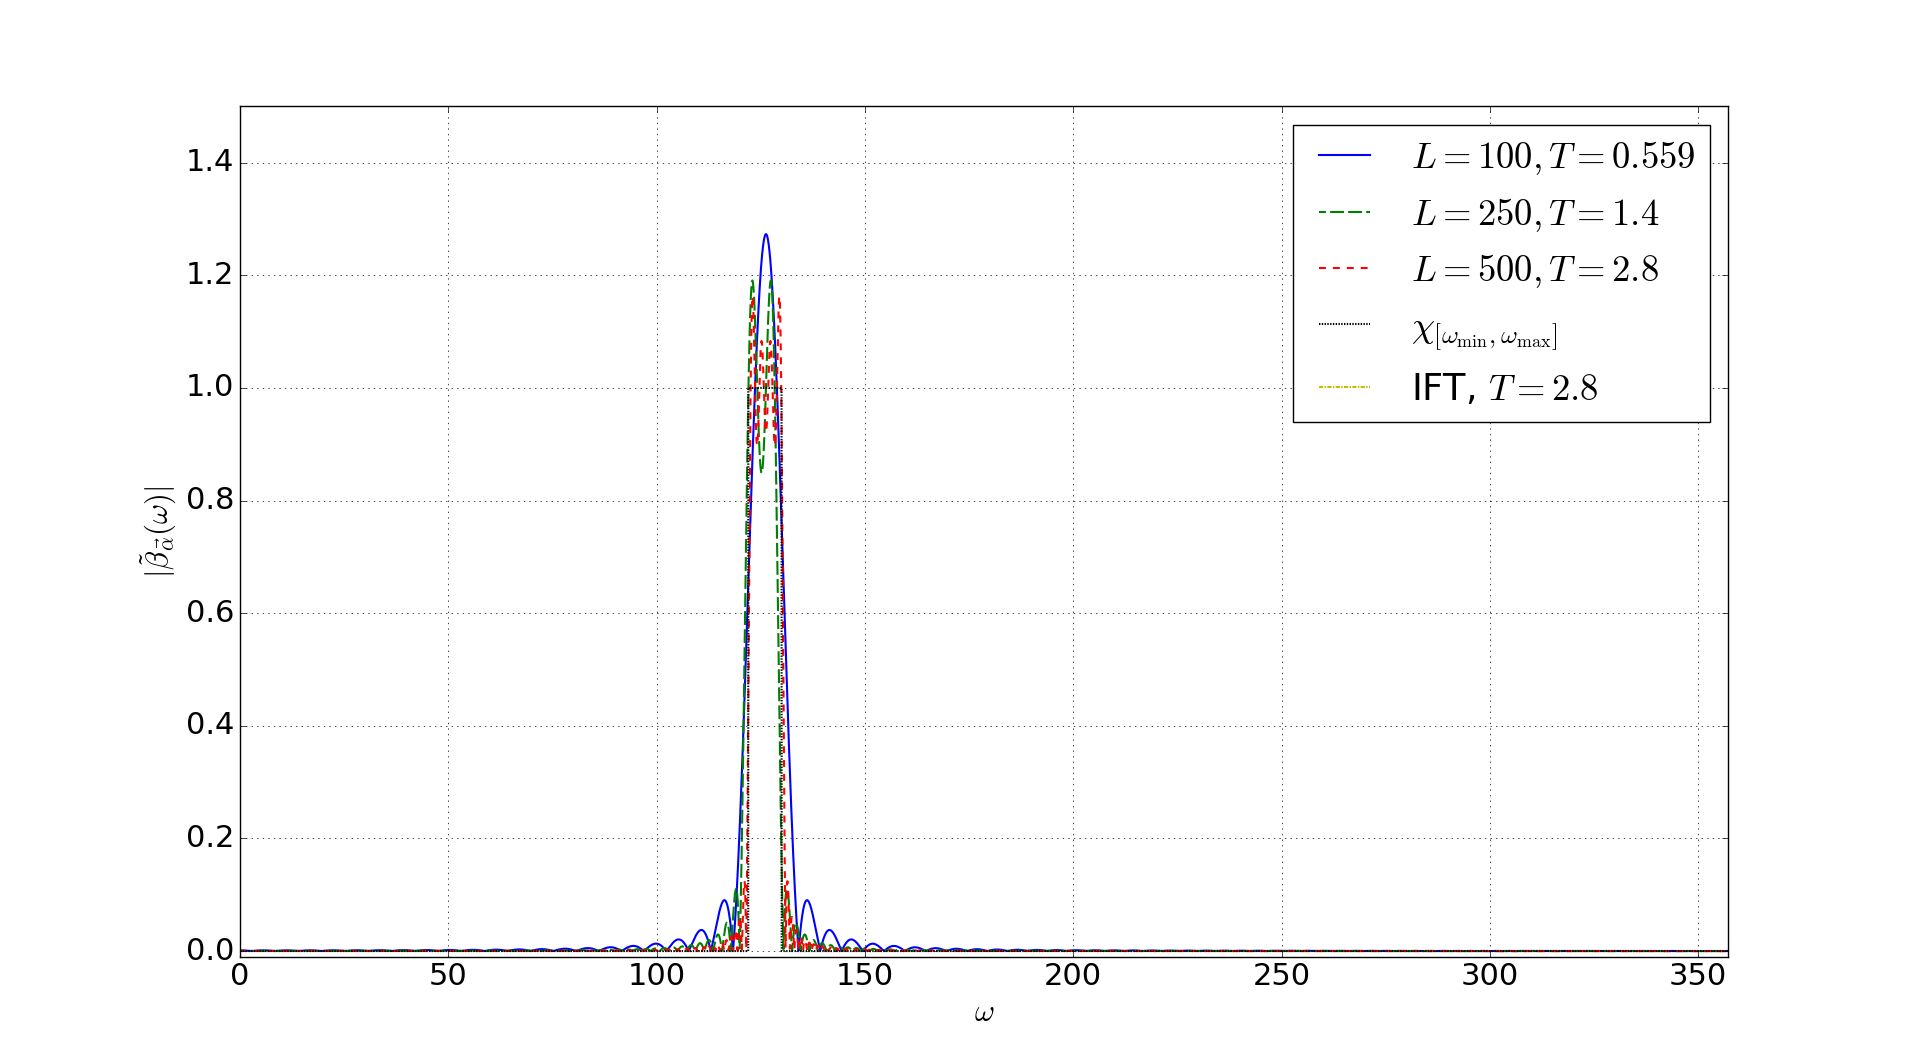
\includegraphics[width=0.75\linewidth]{latex//images//fourier/Figure_3.png}
    \caption{Plots of function $\left|\dff(\omega) \right|$ with weight function $\alpha$ obtained by truncated inverse Fourier transform \eqref{eq:alpha fourier}. Target interval $\left[\omega_{\min}, \omega_{\max} \right] = [3, 6]$, time-step $\tau = 0.0056$, $\omega_\e = 2/\tau \approx 357.14$ and varying number of time-steps $L$. }
    \label{fig:fourier1}
\end{figure}
\begin{figure}
    \centering
    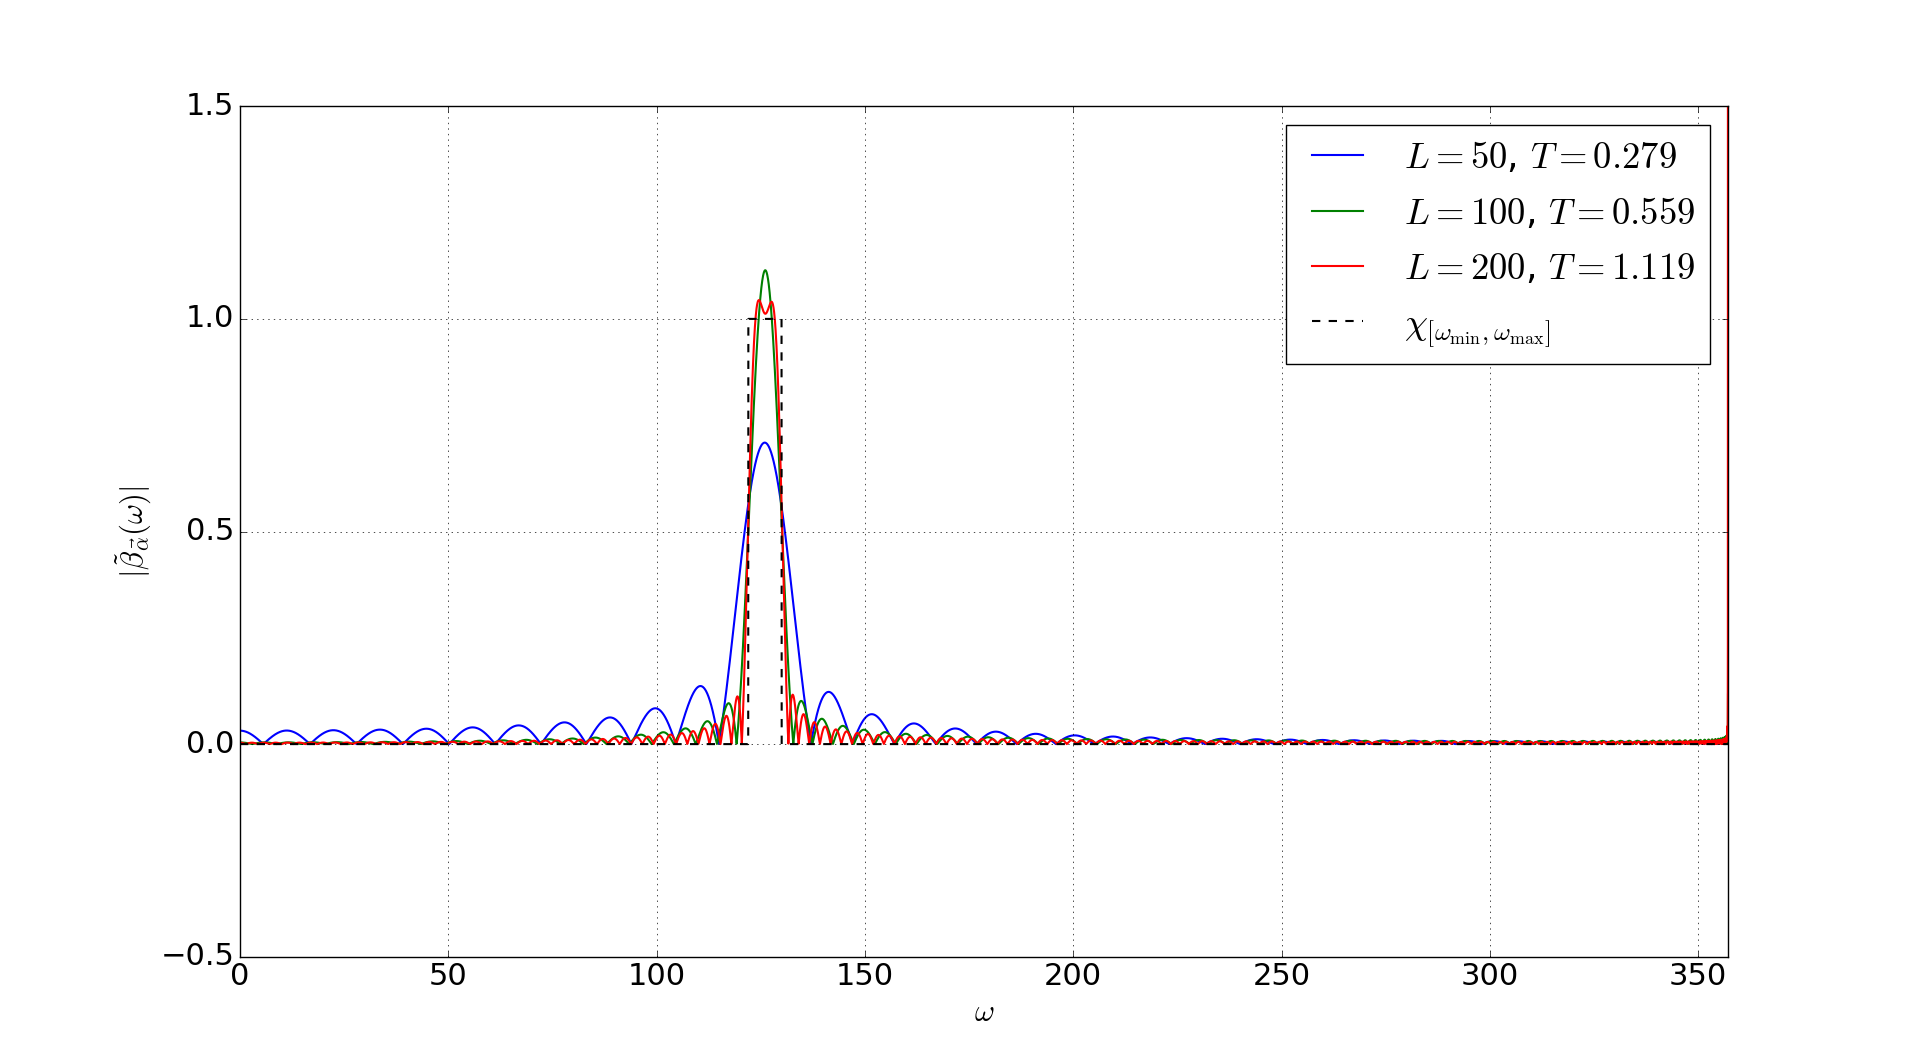
\includegraphics[width=0.75\linewidth]{latex//images//fourier/Figure_4.png}
    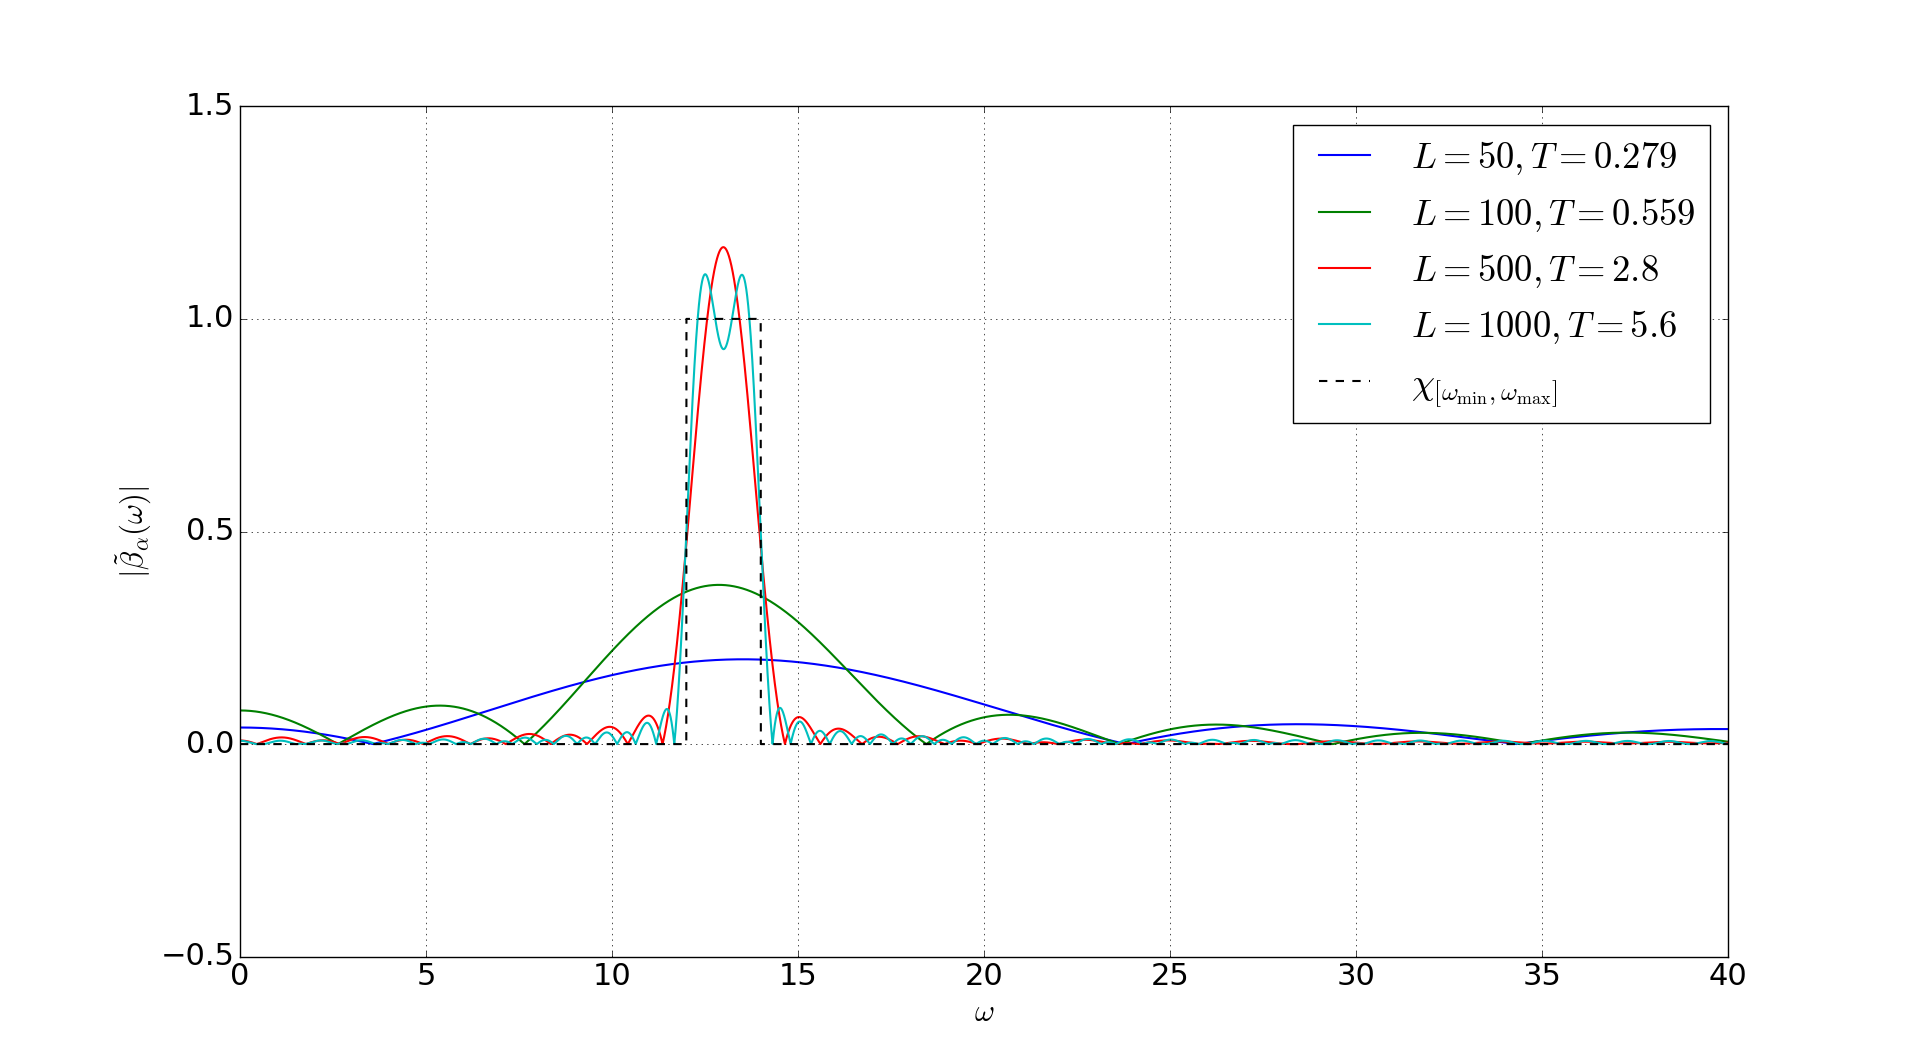
\includegraphics[width=0.75\linewidth]{latex//images//fourier/Figure_5.png}
    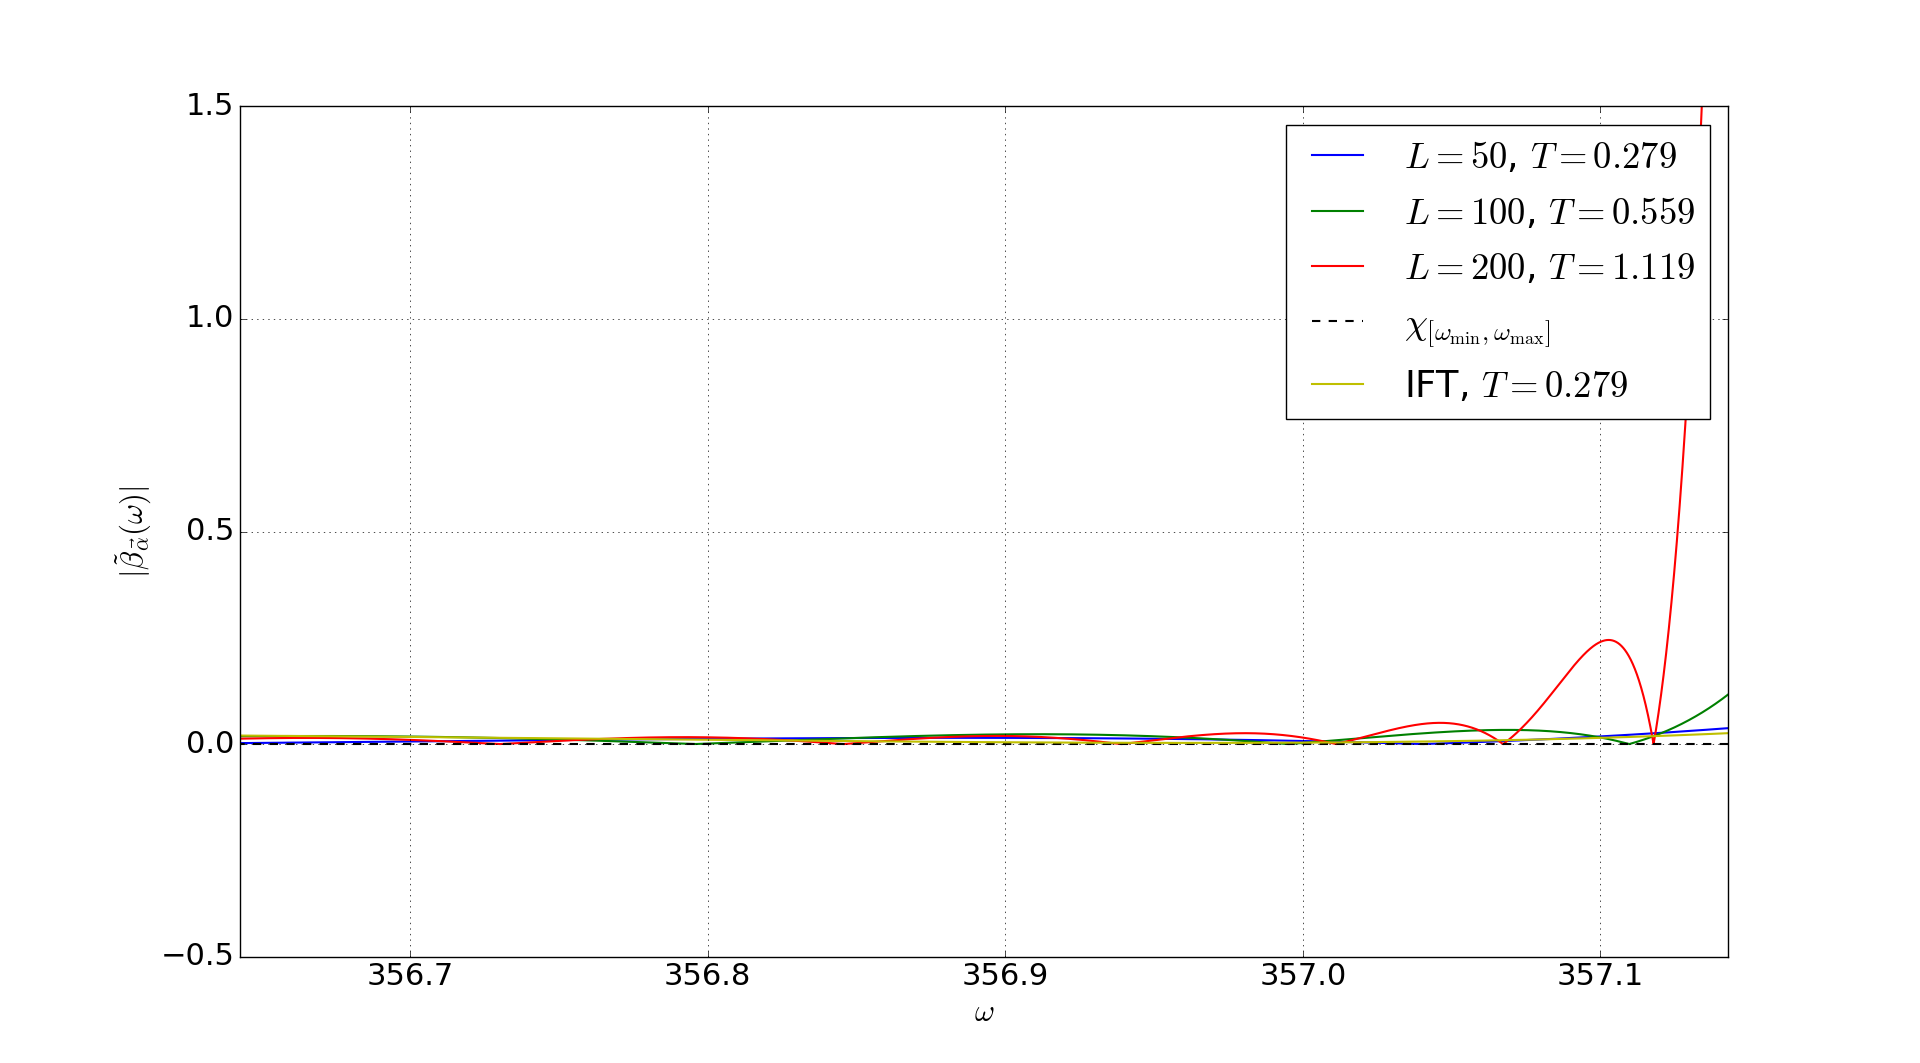
\includegraphics[width=0.75\linewidth]{latex//images//fourier/Figure_6.png}
    \caption{Plots of function $\left|\dff(\omega) \right|$ with weight function $\alpha$ obtained by truncated inverse Fourier transform \eqref{eq:alpha fourier}. Target interval $\left[\omega_{\min}, \omega_{\max} \right] = [12, 14]$, time-step $\tau = 0.0056$, $\omega_\e = 2/\tau \approx 357.14$ and varying number of time-steps $L$. }
    \label{fig:fourier2}
\end{figure}

\section{Collocation method}\label{section:collocation}
The definitions of the discrete operator $C$ for Krylov iteration \eqref{eq:C operator} and of the discrete filter function $\dff$ \eqref{eq:dff} for fixed time-step $\tau$ and number of time-steps $L$ does not require the values of the weight function in the whole domain, but only in $\tau l$ for $l=0, \dots, L-1$. Thus we can reduce the problem to find a vector $\Vec{\alpha} \in \R^L$, such that $\Vec{\alpha}_l = \alpha(\tau l)$ for all $l=0, \dots, L-1$.

Following definition is analogous to the previous definition of the discrete filter function.

\begin{definition}
    Let $\tau > 0$ be the time-step, $L\in \N$ be the number of time-steps and let $q_l(\omega)$ be defined for all $l \in \N$ and $\omega \in \R$ by \eqref{eq:q def}. Let $\Vec{\alpha}\in\R^L$ be a weight vector. Then the discrete function $\dffv: [0, \infty) \rightarrow \R$ is defined as:
    \begin{equation*}\label{eq:dffv}
        \dffv (\omega) := \tau \left(q_0(\omega), \dots, q_{L-1}(\omega)\right) \Vec{\alpha}. 
    \end{equation*}
\end{definition}

As target function we take again indicator $\chi_{\left[\omega_{\min}, \omega_{\max}\right]}$. We select $L$ nodes in the controlled interval, in simplest setting equidistant, and formulate our problem as a polynomial collocation problem with $\left\{q_l : l=0, \dots, L-1\right\}$ basis of the space of polynomials up to degree $L-1$ in $\omega^2$.
\begin{definition}\label{def:evaluation matrix}
    For given number of time-steps $L\in \N$ and $K\in \N$ collocation nodes $ 0 = \omega_0 < \dots < \omega_{K-1}$ we define the evaluation matrix $Q \in \R^{K\times L}$ as $Q_{kl} := q_l\left(\omega_k\right)$ for all $k=0, \dots, K-1$ and $l=0, \dots, L-1$. 
\end{definition}

Let $\tau>0$ be the time-step and $L\in \N$ be the number of time-steps and $\left[\omega_{\min}, \omega_{\max}\right]$ be the target interval. Selecting $L$ equidistant collocation nodes $\omega_l = l\omega_\e/ (L-1)$ for $l=0, \dots, L-1$ in controlled interval $\left[0, \omega_{\e}\right]$ leads to collocation problem to find $\Vec{\alpha} \in \R^L$, such that:
\begin{equation*}
    \forall k = 0, \dots, L-1: \quad \dffv\left(\omega_k\right) = \chi_{\left[\omega_{\min}, \omega_{\max}\right]}(\omega_k).
\end{equation*}
This problem is equivalent to linear system of equations:
\begin{equation}\label{eq:alpha eq coll}
     Q \Vec{\alpha} = \frac{1}{\tau} \left(\chi_{\left[\omega_{\min}, \omega_{\max}\right]}(\omega_k) \right)_{k=0}^{L-1}
\end{equation}
with matrix $Q$ from Definition \ref{def:evaluation matrix}.

As example we choose same parameters as in the previous section. Plots of obtained discrete filter functions for two values of $L = 10 $ and $L=25$ are in the Figure \ref{fig:eq coll beta}. We solve the system of linear equations \eqref{eq:alpha eq coll} with \texttt{numpy.linalg.solve()} function in Python. 

\begin{figure}
    \centering
    \includegraphics[width=0.75\linewidth]{latex//images//equi_coll/Figure_1.png}
    \caption{Plot of function $\left|\dffv\right|$ with $\Vec{\alpha}$ obtained by collocation \eqref{eq:alpha eq coll}. Target interval $\left[\omega_{\min}, \omega_{\max} \right] = [39, 45]$, time-step $\tau = 0.0056$, $\omega_\e = 2/\tau \approx 357.14$ and varying number of time-steps and collocation nodes $L$. Crosses represent values of the target function in knots. }
    \label{fig:eq coll beta}
\end{figure}

By small number of collocation knots, intervals between nodes are large and we can observe strong oscillation of the polynomial for larger values of $\omega$. Increasing number of nodes does not improve the behaviour for two reasons. Firstly, this increases degree of the polynomial, what compounds the problem despite shorter intervals between nodes. Secondly, higher values of $L$ rapidly worsen conditioning of the matrix $Q$. Figure \ref{fig:eq coll cond} presents $\mathrm{cond}(Q) := \|Q\|_2 \|Q^{-1}\|_2$ (where $\| \cdot \|_2$ denotes induced matrix norm by the euclidean norm) depending on size of the problem $L$.

\begin{figure}
    \centering
    \includegraphics[width=0.75\linewidth]{latex//images//equi_coll/Figure_2.png}
    \caption{Condition number of the evaluation matrix $Q$ (matrix norm induced by euclidean norm) depending on number of collocation nodes $L$.}
    \label{fig:eq coll cond}
\end{figure}


\bibliographystyle{alpha} 
%\bibliographystyle{abbrv}
\bibliography{literature.bib}

\end{document}
